\chapter{Classification Method} \label{chap:kitt_nn}
Principles of feedforward neural networks, based on the perceptron idea (see [ref to lit]), are used for developing a new classification framework.

As the first part of the study is devoted to the evolution of a new network pruning algorithm, besides some standard functions, the new framework implementation must be capable of:

\begin{enumerate}
\item pruning of the network during training process;
\item retraining the pruned network.
\end{enumerate}

In this thesis, the implemented neural network framework is called \textit{kitt\_nn}. Implementation details are described in \cref{sec:implementation_of_nn}.

\section{Network Structure} \label{sec:network_structure}
In this work, a \textit{feedforward} neural network is used, where none of the neurons are connected to other neurons in the same layer or any neurons in the previous layers and are connected to all neurons in the following layer (\cref{img:neural_net}).

\begin{figure}[H]
  \centering
  \includegraphics[width=0.8\textwidth]{neural_net.png}
  \caption{Structure of a feedforward neural network}
  \label{img:neural_net}
\end{figure}

As the number of neurons in input and output layers are determined by a chosen dataset, the network structure is defined by:
\begin{enumerate}
\item number of hidden layers;
\item number of neurons in each of the hidden layers.
\end{enumerate}

\section{Neuron Principle} \label{sec:neuron_principle}
The behaviour of artificial neurons follows our understanding of how biological neurons work. One unit consists of multiple inputs and a single output. A model of neuron is shown in \cref{img:model_neuron}. The diagram complies with the following notation:

\begin{description}
\item[$ a_k^{(i)} $] : activity of $ k^{th} $ neuron in $ i^{th} $ layer
\item[$ w_{l, k}^{(i)} $] : weight of synapse connecting $ l^{th} $ neuron in $ i^{th} $ layer with $ k^{th} $ neuron in $ (i+1)^{th} $ layer
\item[$ neuron_k^{(i)} $] : $ k^{th} $ neuron in $ i^{th} $ layer
\item[$ b_k^{(i)} $] : bias connected to $ k^{th} $ neuron in $ i^{th} $ layer
\item[$ z_k^{(i)} $] : activation of $ k^{th} $ neuron in $ i^{th} $ layer
\item[$ f() $] : transfer function (\cref{eq:nn_transfer_function})
\end{description}

\begin{figure}[H]
  \centering
  \includegraphics[width=0.9\textwidth]{neuron_principle.png}
  \caption{A model neuron}
  \label{img:model_neuron}
\end{figure}

Assuming $ p $ being the number of neurons in $ i^{th} $ layer, the activation of $ neuron_k^{(i+1)} $ is computed as in \ref{eq:neuron_activation}

\begin{align} \label{eq:neuron_activation}
neuron_k^{(i+1)} = \displaystyle{\sum_{l=1}^{p} a_l^{(i)} \cdot w_{l,k}^{(i)}} + b_k^{(i+1)}
\end{align}

The sigmoid function given as in \cref{eq:nn_transfer_function} is used as the transfer function for computing the activities of individual neurons.

\begin{align} \label{eq:nn_transfer_function}
f(z) = \frac{1}{1 + e^{-z}}
\end{align}

The sigmoid function maps neuron activations into $ [0.0, 1.0] $ interval. This approach is used for most of the work in this study. Additionaly, the \textit{tanh(z)} function is implemented (compared to \textit{sigmoid(z)} in \cref{fig:transfer_functions}), in order to test one of the pruning methods based on weights sensitivity (discussed later). The \textit{tanh(z)} function maps the input \textit{z} into $ [-1.0, 1.0] $ interval.

\begin{figure}[H]
  \centering
  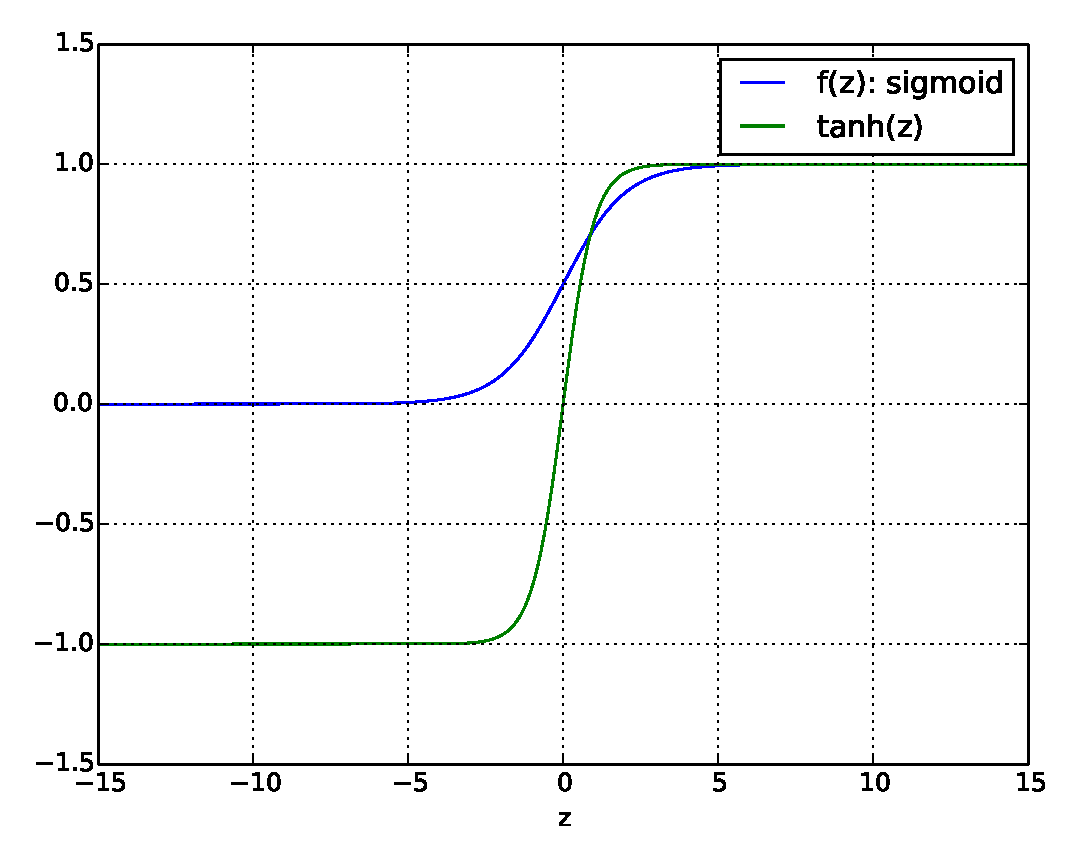
\includegraphics[width=0.5\textwidth]{transfer_functions}
  \caption{Used transfer functions: sigmoid and tanh}
  \label{fig:transfer_functions}
\end{figure}

\section{Learning Algorithm for Network Training} \label{sec:learning_algorithm}
In general, learning algorithms represent the part of artificial systems that makes them behave intelligently when accomplishing a specific task. In classification, the goal of learning is to fit some training data to a model, which generally means to set some parameters based on the chosen classification approach.

\begin{figure}[H]
  \centering
  \includegraphics[width=0.82\textwidth]{backpropagation.png}
  \caption{Training process flowchart. $ T_1 $: Threshold for a terminating condition based on a learning error. If the error is reduced to be lower than this threshold, the learning process is stopped. $ T_2 $: Threshold for a terminating condition based on number of iterations (epochs). The learning process is stopped after a specified number of epochs, no matter how successful the training has been.}
  \label{img:backpropagation}
\end{figure}

In case of feedforward neural networks, the learning goal is to find optimal values for two groups of parameters - \textit{weights} and \textit{biases} (described in \cref{sec:intro_to_nn}).

A popular algorithm called \textit{Backpropagation} is used to deal with the learning task. The backpropagation abbreviation stands for \textit{backward propagation of errors}. The approach is based on an optimization method called \textit{Gradient Descent Algorithm (GDA)}.

In this work, the implementation is made to be compatible with the \textit{kitt\_nn} network (\cref{sec:implementation_of_nn}) and adjusted to the needs of the developed pruning algorithm (\cref{sec:network_pruning_algorithm}). The learning process is summarized by the flowchart in \cref{img:backpropagation}. The procedure follows algorithmical steps found in \citep{online:nn_demystified}.

\subsection{Using Mini-batches} \label{ssec:minibatches}
The training procedure of multilayer perceptrons ([ref to lit]) is based on propagating one sample at a time through a network. However, more samples can be send to the network, while activities and activations of neurons in one layer are computed at the same time for all of those samples.

This group of samples is called \textit{a mini-batch}. Using mini-batches can speed up the process, however, it can bring some problems with finding the right solution by the \textit{Gradient Descent} method (evident from \cref{eq:batch_gd}). Usually, the mini-batch size is left as a training parameter. In this work, it is set to \textit{10}.

\subsection{Matrix Notations} \label{ssec:matrix_notation}
Assuming feedforward neural networks and reffering to \cref{img:model_neuron}, the following notation is used for multiple samples processing.

\begin{description}
\item[$ X $] : network input: $ m $-by-$ n $ matrix, where $ m $ is the number of samples and $ n $ is the size of one sample
\item[$ W^{(i)} $] : $ p $-by-$ r $ matrix of weights for synapses from neurons in layer $ i $ (layer of $ p $ neurons) to neurons in layer $ (i+1) $ (layer of $ r $ neurons)
\item[$ B^{(i)} $] : vector of length $ p $ including biases for neurons in layer $ i $ (layer of $ p $ neurons)
\item[$ Z^{(i)} $] : $ r $-by-$ m $ matrix of activations for neurons in layer $ (i) $ (layer of $ r $ neurons), $ m $ is the number of processed samples
\item[$ A^{(i)} $] : $ r $-by-$ m $ matrix of activities of neurons in layer $ (i) $ (layer of $ r $ neurons), $ m $ is the number of processed samples
\item[$ \hat{y} $] : network predicted output: $ q $-by-$ m $ matrix, where $ q $ is the number of output neurons and $ m $ is the number of processed samples ($ \hat{y} = f(Z^{(j)}) $, where $ j $ is the number of layers)
\item[$ y $] : network actual output (known targets): $ q $-by-$ m $ matrix, where $ q $ is the number of output neurons and $ m $ is the number of processed samples
\item[$ \delta^{(i)} $] : error vector of length $ p $ for $ p $ neurons of $ i^{th} $ layer
\end{description}

\subsection{Forward Propagation} \label{ssec:forward_propagation}
With reference to the previous sections, the following equations are used to propagate a batch of samples $ X $ through a network and get a corresponding matrix of outputs $ \hat{y} $.

\begin{align}
Z^{(2)} = X \cdot W^{(1)} + B^{(2)}
\end{align}

\begin{align}
Z^{i+1} = A^i \cdot W^i + B^{(i+1)}
\end{align}

\begin{align}
A^{(i)} = f(Z^{(i)})
\end{align}

\begin{align}
\hat{y} = f(Z^{(j)})
\end{align}

\subsection{Error Calculation} \label{ssec:error_calculation}
To get an idea about how wrong the networks predictions are, the network needs a teacher. For this reason the learning is called \textit{supervised}, as there is a batch of training data with known targets. Comparing the predictions with the correct targets, one can calculate a prediction error. 

The prediction error of the propagated batch of samples is expressed as a cost function $ J $. The goal is to minimize $ J $.

\begin{align} \label{eq:cost_function}
J = \displaystyle{\sum_{k=1}^m} \frac{1}{2}(y_k - \hat{y}_k)^2
\end{align}

\subsection{Parameter Update} \label{ssec:parameter_update}
Knowing the prediction error, the goal of the learning algorithm is to update the network weights and biases in order to reduce the error for next prediction.  It is known, that some combination of the parameters makes $ J $ (\cref{eq:cost_function}) minimal. There is no chance to check all possible combinations for bigger networks, therefore \textit{GDA} is used here.

Partial derivatives $ \frac{dJ}{dw} $ for all weights $ w $ of chosen weight matrix $ W^{(i)} $ belonging to layer $ i $ are computed and set equal to zero ($ \frac{dJ}{dw} = 0 $). Applying this on a mini-batch, we get $ m $ derivatives $ (\frac{dJ}{dW^{(i)}})_k $ for $ m $ input samples. 

\textit{GDA} is then applied on the summation of these derivatives and so all examples are considered as one (\cref{eq:batch_gd}). In other words, one can understand it as every sample has a vote on how to find the minimal error and the result is obtained as a compromise.

\begin{align} \label{eq:batch_gd}
\frac{dJ}{dW^{(i)}} =  \displaystyle{\sum_{k=1}^m} (\frac{dJ}{dw})_k
\end{align}

Having several layers of a network results in several weights (and biases) mattrices, while the goal is to find optimal parameters of overall network. In order to compute optimal parameters in all of the mattrices, the sum rule in differentation (\cref{eq:sum_rule}) followed by the chain rule (\cref{eq:chain_rule}) are applied.

\begin{align} \label{eq:sum_rule}
\frac{\delta}{\delta x} (u+v) = \frac{\delta u}{\delta x} + \frac{\delta v}{\delta x}
\end{align}

\begin{align} \label{eq:chain_rule}
(f \circ g)' = (f' \circ g) \cdot g'
\end{align}

Due to these properties, the error obtained at the network output (\cref{ssec:error_calculation}) is propagated backwards layer by layer through the network (\cref{eq:error_backprop}) and derivatives $ \frac{dJ}{dW^{(i)}} $ for all $ i $ layers are found (\cref{eq:part_derivative}). For this procedure, the derivative of our transfer function is needed (\cref{eq:nn_transfer_function_der}).

\begin{align} \label{eq:nn_transfer_function_der}
f'(z) = f(z) \cdot (1-f(z))
\end{align}

\begin{align} \label{eq:error_backprop}
\delta^{(i)} = \delta^{(i+1)} \cdot (W^{(i)})^T \cdot f'(Z^{(i)})
\end{align}

\begin{align} \label{eq:part_derivative}
\frac{dJ}{dW^{(i)}} = (a^{(2)})^T \cdot \delta^{(i+1)} \qquad\qquad \frac{dJ}{dB^{(i)}} = \delta^{(i+1)}
\end{align}

The parameters are then updated for the next iteration as shown in \cref{eq:params_update}.

\begin{align} \label{eq:params_update}
W_{(t+1)}^{(i)} = W_{(t)}^{(i)} + \frac{dJ}{dW^{(i)}}_{(t)} \qquad\qquad B_{(t+1)}^{(i)} = B_{(t)}^{(i)} + \frac{dJ}{dB^{(i)}}_{(t)}
\end{align}

In this work, the learning algorithm is implemented in \textit{Python}, using mostly the \textit{numpy} library for the expensive matrix operations. The implementation complies with the needs of the pruning algorithm from \cref{sec:network_pruning_algorithm} and is fully compatible with the \textit{kitt\_nn} framework for any type of data.

\section{Network Pruning Algorithm} \label{sec:network_pruning_algorithm}
The network pruning algorithm (PA) is the novelty of this study. The state-of-the-art methods based on feedforward neural networks (see \cref{sec:intro_to_nn}) use a fully-connected structure by default. This means that each unit is connected to all units in the next layer. Hence a net structure is defined just by the number of hidden layers and the number of neurons in each of those. The question is if all of by default generated connections are significant and necessary for classification.

\subsection{Pruning Method} \label{ssec:pa_method}
The hypothesis is that some synapses of a fully connected feedforward network can be removed without the net's classification performance being influenced significantly.  The problem is graphically illustrated in \cref{img:pruning_problem_formulation}.

\begin{figure}[H]
  \centering
  \includegraphics[width=1.0\textwidth]{pruning_problem_formulation.png}
  \caption{Pruning Algorithm: hypothesis formulation}
  \label{img:pruning_problem_formulation}
\end{figure}

The task is to identify the unimportant synapses. The basic idea of the algorithm is as follows:
\begin{enumerate}
\item a fully-connected network is initialized and trained on some data in order to reach as high accuracy as possible;
\item some of the synapses are removed and a classification ability of the pruned net is tested;
\item if it has not dropped significantly, the removed synapses were unimportant
\end{enumerate}

The way of removing synpases is called \textit{pruning algorithm (PA)}.

The idea behind the PA implemented in this study is based on weight changes during the network training. It is expected that a synapse, whose weight does not evolve while the network is trained, does not contribute to classification much. 

\subsection{Algorithm Realization} \label{ssec:pa_realization}
The pruning algorithm itself is an iterative process, however, as shown in \cref{img:pa_flowchart}, two important steps are done in advance.

\begin{figure}[H]
  \centering
  \includegraphics[width=0.9\textwidth]{pa_flowchart.png}
  \caption{Overall flowchart of the pruning process}
  \label{img:pa_flowchart}
\end{figure}

First of all, the following variables are initialized:

\begin{description}
\item[net] : a fully-connected \textit{kitt\_nn} \textit{Network()} with an oversized structure (many hidden neurons) and randomly set weights and biases
\item[percentile] : algorithm variable, set to $ 75 $ by default
\item[percentile levels] : array of final variables, set to $ [75, 50, 20, 5, 1] $ by default
\item[required accuracy] : required classification accuracy for a chosen problem (e.g. 0.95)
\item[stability threshold] : if the classification does not improve over several learning iterations, this is the number of stable iterations to terminate the training after
\end{description}

Additionally, some standard learning parameters like the \textit{learning rate}, \textit{number of epochs} and \textit{mini-batch size} can be set and, of course, a dataset is chosen.

Once the initialization is done, the network is trained with some optimal learning parameters until it reaches the required classification success rate. As mentioned above, the pruning algorithm is based on weight changes. Therefore, the initial weights for synapses are kept. Then, the trained network is passed to the pruning phase, which is shown in \cref{img:pruning_algorithm}.

\begin{figure}[H]
  \centering
  \includegraphics[width=0.8\textwidth]{pruning_algorithm.png}
  \caption{The Pruning Algorithm: initialized variables are in bold, red marked functions reffer to \ref{img:cut_synapses} and \ref{img:accuracy_kept} respectively}
  \label{img:pruning_algorithm}
\end{figure}

Initially, a backup of the current network structure is made by creating a network copy. The pruning is then performed using this copy. The pruning method is shown in \cref{img:cut_synapses}.

\begin{figure}[H]
  \centering
  \includegraphics[width=0.75\textwidth]{cut_synapses.png}
  \caption{Synaptic pruning based on weight changes and current percentile value}
  \label{img:cut_synapses}
\end{figure}

As discussed above, an initial weight value was saved for each synapse before the training. Hence, for $ n $ being the total number of synapses, weight changes $ \Delta w_i $ are known (\ref{eq:weight_change}).

\begin{align} \label{eq:weight_change}
\Delta w_i = |w\_init_i - w\_current_i|, \quad i = 1, ..., n
\end{align}

Based on these changes and on the current $ percentile $ value, a threshold ($ th $ in \cref{img:cut_synapses}) is determined. Then, all synapses with a lower change in weight than this threshold are removed, and, if there is a neuron with no connections left, it is removed as well.

If the $ percentile $ variable has been decreased so that it equals zero, the threshold is set to the minimum of all weight changes. In this case, only one synapse is then removed at a time.

\begin{figure}[H]
  \centering
  \includegraphics[width=0.75\textwidth]{accuracy_kept.png}
  \caption{Evaluation of the classification accuracy after pruning}
  \label{img:accuracy_kept}
\end{figure}

After cutting some synapses, the network is checked for keeping the required classification accuracy as shown in \cref{img:accuracy_kept}.

The evaluation is performed by testing the network on validation data. If the classification accuracy has dropped, the network is retrained using training data of the dataset.

If the classification accuracy has been kept after the pruning, the current net structure is saved and considered as a reference for the next pruning loop.

If it is not possible to retrain the pruned net and to reach the required accuracy, two possibilities arise:

\begin{enumerate}
\item Only one synapse has been removed during the last pruning step and the accuracy has been broken. This means that even this single synapse with the least change in weight is important for classification. Therefore, the pruning is stopped and the current net structure (including this last synapse) is saved as the minimal structure.
\item More synapses have been removed during the last pruning step, and this broke the accuracy. In this case, the percentile level is decreased (based on the initialized array of percentile levels) and so less synapses are removed during the next pruning iteration.

In this manner, at some point of the pruning process, the algorithm will come to removing only one synapse at once and then, finally, only case 1 will remain.
\end{enumerate}

Therefore, the algorithm is finite. Moreover, it guarantees that the classification success rate does not drop. It is evaluated in detail and compared to some other approaches from \citep{article:10:pa}; (also discussed in \cref{sec:pruning_algorithms}) in the results part (\cref{sec:pruning_algorithm_results}).

\subsection{Datasets for Evaluation of the Pruning Algorithm} \label{ssec:testing_datasets}
Two datasets were used for verification of the pruning algorithm: XOR and MNIST. Those are introduced in the following sections and the evaluation is presented in section X.

The pruning algorithm was also applied on the terrain classification problem (evaluated in section X).

\subsubsection*{XOR Dataset}
This dataset relates to the well-known XOR problem defined by a thruth table (\cref{tab:xor}).

\begin{table}[H]
\centering
\caption{XOR problem definition}
\label{tab:xor}
\begin{tabular}{|c|c|c|}
\hline
$ \mathbf{x_1} $ & $ \mathbf{x_2} $ & \textbf{y} \\ \hline
0           & 0           & 0          \\ \hline
0           & 1           & 1          \\ \hline
1           & 0           & 1          \\ \hline
1           & 1           & 0          \\ \hline
\end{tabular}
\end{table}

Formulating the XOR gate as a classification problem, it is represented by two linearly inseparable classes with labels $ 0 $ and $ 1 $. In this case, each class consists of $ 1000 $ samples, which have been generated using the developed GUI (\cref{sec:gui}). The composition of the two classes in a 2D space is shown in \cref{img:data_xor}.

\begin{figure}[H]
  \centering
  \includegraphics[width=0.5\textwidth]{data_xor.png}
  \caption{2D XOR Data illustration}
  \label{img:data_xor}
\end{figure}

The points (samples) have been generated pseudo-randomly, while it is guaranteed that the 'red' samples are distributed half-and-half between the two 'red' areas. The minimal distance between a 'blue' and a 'red' sample is $ 0.001 $ and it is possible to separate the classes using two lines.

The XOR dataset is essential for evaluation of the implemented PA, as the minimal network structure capable of solving the problem is known. There are two structures (\cref{img:xor_min}), both considered as minimal. Geometrically, the version shown in \cref{img:xor_min1} creates the two lines in 2D space to separate the classes, while the second one (\cref{img:xor_min2}) transfers the problem from 2D space into 3D space and creates a separation plane.

\begin{figure}[H]
\centering
\begin{subfigure}{.5\textwidth}
  \centering
  \includegraphics[width=.8\linewidth]{xor_min1.png}
  \caption{Minimal structure 1}
  \label{img:xor_min1}
\end{subfigure}%
\begin{subfigure}{.5\textwidth}
  \centering
  \includegraphics[width=.8\linewidth]{xor_min2.png}
  \caption{Minimal structure 2}
  \label{img:xor_min2}
\end{subfigure}
\caption{XOR Dataset: minimal network structures}
\label{img:xor_min}
\end{figure}

The goal of the pruning algorithm is to end up with a network of the structure in \cref{img:xor_min1}, when the network is initially oversized. The evaluation is presented in \cref{ssec:evaluation_on_xor}.

\subsubsection*{MNIST Dataset}
The second testing problem is the well-known classification of handwritten digits. The dataset is provided by \citep{online:mnist}. Some examples of digit samples are shown in \cref{img:data_mnist}.

\begin{figure}[H]
  \centering
  \includegraphics[width=0.4\textwidth]{data_mnist.png}
  \caption{MNIST Data illustration \citep{online:mnist}}
  \label{img:data_mnist}
\end{figure}

The dataset has a training set of $ 60,000 $ examples (later split into $ 50,000 $ training and $ 10,000 $ validation examples), and a test set of $ 10,000 $ examples. The digits have been size-normalized and centered in a fixed-size image.

In this case, the minimal network structure is not known. On the other hand, detailed results of classification accuracy for various classifiers are provided, which is good for comparison.

\subsection{Using Network Pruning for Feature Selection} \label{ssec:minimal_structure_util}
In general, only the number of neurons (inputs and outputs) is determined for a chosen dataset. The pruning algorithm brings an additional information about the hidden part of the network. A minimal network structure is obtained as the PA outcome. This means that all the neurons and synapses contained in the network are important for classification.

Knowing that each of these units takes a part and is not useless, one can ask what role a single neuron/synapse has with respect to the chosen dataset.

This can be investigated by tracking the connections from the input to the output layer. Based on this approach, one can find some correlations between the feature selection of input vectors and the selected output class (demonstrated on a MNIST example in \cref{img:structure_util}). Evaluation on MNIST dataset is shown in \cref{sssec:mnist_analysis}.

\begin{figure}[H]
  \centering
  \includegraphics[width=0.55\textwidth]{min_structure_analysis.png}
  \caption{Analysis of the minimal structure examplified on digit 5 (MNIST dataset)}
  \label{img:structure_util}
\end{figure}

\section{Graphical User Interface} \label{sec:gui}
The graphical interface has been implemented as an extension for \textit{kitt\_nn} framework. It is actually not strictly needed for this study, but it provides some interesting functions, which are worth being introduced. Anyway, any type of visualization usually helps to understand a problem better.

\begin{figure}[H]
  \centering
  \includegraphics[width=1.0\textwidth]{gui_screen.png}
  \caption{Screenshot of the graphical user interface}
  \label{img:gui_screen}
\end{figure}

This GUI is capable of:
\begin{enumerate}
\item Loading a dataset in a specific form and, if possible, visualizing it (see XOR data in \cref{img:data_xor} for an example, this image is generated by the GUI).
\item Generating a network of any hidden structure. The input and output layers are defined by the chosen dataset. The network is then visualized (as shown in \cref{img:gui_screen}).
\item Removing synapses of the network, while the visualization is interactive with the structure changes.
\item Training the network, while the visualization is interactive, so the weights changes can be seen online.
\item Performing some tests and plotting basic evaluations.
\item Adjusting the visualization view in sense of zooming, resizing or changing colors.
\end{enumerate}

The visualization is not that useful for huge network structures, however, it can be essential at some points of the workflow. Nevertheless, it is considered as the very fist version for now and aimed to be upgraded in the future.